\documentclass[thesis]{subfiles}

\begin{document}
%*******************************************************************************
%*********************************** Future Work *****************************
%*******************************************************************************

\chapter{Future Work}  %Title of the First Chapter
\label{futurework}

%********************************** %First Section  **************************************

Research outcomes are often better evaluated by the questions borne rather than the questions answered. In this section I'll address the main research questions I believe my work has highlighted, and propose future directions for research I believe would have the most impact on the field.

\section{End-to-End Learning?}
Classic computer vision approaches depended on hand-designing problem specific \emph{features} --- salient representations of the input --- requiring expert knowledge of the domain, limiting the scalability and effectiveness of this approach. Early computer vision research, for example, depended on finding prominent edges in images. The appeal of deep learning, as compared to classic feature-driven approaches in computer vision (and speech recognition, etc), is that neural networks are trained \emph{end-to-end}. Whereas in classic computer vision, more salient representations of the input must be hand-designed for each problem, deep learning algorithms can be trained directly on the original data itself, and have been shown to learn better representations of the data.

\begin{figure}[tbp]
	\centering
	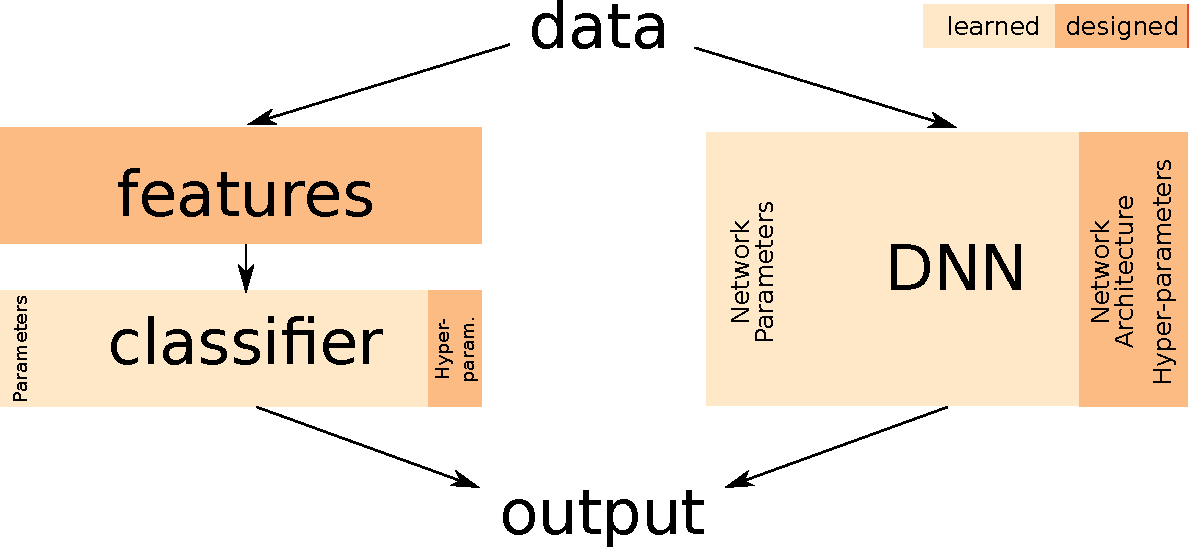
\includegraphics[width=0.66\textwidth]{dnnvsfeatures}
	\caption{A comparison of classic feature-based approach to computer vision, and deep learning approaches. Although both methods require hand-tuned hyper-parameters and design, deep learning methods avoid much of the hand-engineering of classic approaches.}\label{dnnvsfeatures}
\end{figure}
	
Glossed over in this description of deep learning, as it is often in the field itself, is that this learning ability does not come for free, it relies on very specific assumptions that are mostly encoded in the design of the neural network architecture itself --- what I call \emph{structural priors} --- as necessitated by the Free Lunch Theorem explained in \cref{nofreelunch}. Structural priors require some knowledge of the domain to design but, unlike hand-designed features, are higher level and have broad applicability. In real-world applications fully-connected neural networks are seldom used, every practical application of deep learning has relied on some form of structural prior. \Cref{dnnvsfeatures} illustrates, at a high level, the amount of learning \vs{}design in deep learning as compared to traditional feature-based computer vision.

For example, Convolutional Neural Networks (CNNs) are a broad class of neural network architectures that encode assumptions based on our prior knowledge about learning with natural image inputs. Recurrent Neural Networks (RNNs) are another broad class of architectures that encode our prior knowledge about learning sequence inputs, such as natural language sentences. Neural networks designed with problem-salient structural priors have fewer parameters, are faster, and have better \emph{generalization} --- better accuracy on data outside the training set --- than the fully connected equivalent.

\subsection{Learning Structural Priors}
The move towards ``end-to-end'' learning has made great strides in making learning more automatic, notably in learning complex representations rather than experts designing inferior representations themselves. There still exists however, a significant amount of hand design and manual tuning that is key to the success of any deep learning approach. I hope my work will motivate the field towards a research direction that aims to minimize this further, by working on methods of automatically structuring neural networks, in a move towards a truly ``end-to-end'' learning of DNN structure itself.

The lack of understanding or concrete rules for structuring DNNs means that in practical applications deep learning is often restricted to experts in the field, who have an intuition in network design formed from years of experience, and know which structural priors to use. The effect on deep learning research is no less profound, with a lack of understanding of the basic interplay between structure and learning in DNNs, we have little chance of understanding the limitations of deep learning or the representations learned by the networks. 

The benefits of automatically structuring DNNs go further than these considerations even, as my PhD research has shown, better structured DNNs are more computationally efficient (use fewer parameters and are faster to compute), and generalize better. Currently, training state-of-the-art DNNs for image classification requires a prohibitive amount of time and computational resources --- 3 weeks of training on 8 high-end and expensive graphical processing units (GPUs) --- and yet we know that trained DNNs are very sparse representations and have been shown to be highly compressible. It is because we cannot appropriately understand this sparse structure well enough to fully exploit it that our current DNNs are so inefficient.

With automatic methods of learning the structure, DNNs will become markedly more efficient to train, leading to faster experimental results for research, and also allow easier deployment to embedded devices, such as mobile phones, drones and robots. It would also allow for research strides in learning networks for multiple modalities, for example a self-driving car needs to process input data from normal camera sensors, along with depth maps or point clouds, and even radar. One of the stumbling blocks in doing this is understanding how to best structure a network to deal with multiple inputs which require different structural priors.

Research on finding automatic methods of structuring neural networks is not a completely new avenue of research, with a substantial effort put towards it 30 years ago when neural networks, and datasets, were much smaller. A comprehensive review of the literature is not possible in this short proposal, but suffice to state that there were two main approaches: (i) greedily building networks from scratch, and (ii) pruning (removing parameters) large networks. The proposals made for both building networks from scratch (such as \citep{Fahlman1989}), and pruning full networks (such as \citep{lecun1989optimal}) suffer drawbacks which make them unsuitable in the modern deep network of hundreds of millions of parameters. Even in neural networks of contemporary size, the greedy approach of \citet{Fahlman1989} meant that learned networks were suboptimal. %My proposal should also not be confused with `universal learning', or violating the no free lunch theorem, since we are interested in learning methods for the specific set of problems we as humans are interested in solving, rather than all possible input patterns.

At least three factors prevented this line of research from being successful historically, that I believe have now been overcome. Recent breakthroughs in training DNNs have given us a better understanding of how to train very large, arbitrarily structured networks, notably avoiding the so-called ``vanishing gradient''~\citep{Ioffe2015,He2016}, and a better understanding of initialization~\citep{He2015b}. Extremely large and diverse datasets are now prevalent, such as ImageNet~\citep{ILSVRC2015}, whereas historically datasets were prohibitively small to be useful for automatically structuring DNNs. And finally computational resources have increased dramatically. In fact these are most of the reasons the field of deep learning itself has been more successful now than neural networks were 30 years ago.

\section{Jointly Learning a Basis for Spatial and Channel Extents of Filters}
\label{journalplan}
In the shorter term, there is an obvious question arising from the work presented in \cref{lowrankfilters,deeproots} that explore learning more efficiently by reducing the learned parameters in the spatial and channel extents, respectively, of convolutional filters. These naturally lend themselves to being merged into a single effective method for training with low-rank basis filters. We plan to submit a journal article in which both methods are merged and explored in new results on state-of-the-art deep networks.

\section{Optimization and Structural Priors}
It is notable that many structural priors can be viewed as enforcing sparsity on fully connected networks. For example, in the case of a convolutional neural network (CNN), any learned CNN is representable in a fully connected network, since a CNN can be viewed as a fully-connected network with a specific arrangement of zeroed connect weights, and some duplicated weights (shared weights) as illustrated in \cref{fig:sparseconn}.

The question arises then, why can we not learn these in fully-connected networks? Structural priors give lower training loss, and yet when we optimize 
\mynote{TODO}
\section{Parting Note}
In my PhD I have focused on experiments that I believe shed light on the representations being learned in deep networks. Although the overt motivation of much of the work in its publication has been efficiency, my motivation has always been to show that state-of-the-art deep networks for image classification are over-parameterized and suffer, not only in efficiency, but also in \emph{effectiveness} due to this. Structural priors, such as those demonstrated in this thesis do not only improve the effectiveness of a deep network, but are \emph{required} for good generalization.
\end{document}
